\chapter{Analyse du parcours universitaire des bacheliers (UCAD)}

\section{Introduction}

Ce chapitre s'intéresse à la trajectoire des bacheliers, une fois admis à l'université, en particulier à l'UCAD. 
L’objectif est d’évaluer l’impact des différentes réformes du baccalauréat sur l’orientation et la réussite universitaire des étudiants issus des séries concernées.

Dans un premier temps, nous analyserons l’évolution des effectifs inscrits à l’UCAD selon les séries de baccalauréat impactées par les réformes.
Nous observerons ensuite les établissements et départements universitaires où ces bacheliers sont le plus souvent orientés, afin d’identifier les filières de destination privilégiées selon la série d’origine.

Enfin, une analyse de type \textbf{suivi de cohorte} permettra d’évaluer la progression et les performances académiques de ces étudiants dans le temps (réussite, redoublement, abandon), afin de mieux comprendre les effets des réformes sur la réussite universitaire.

\newpage
\section{Évolution des inscriptions à l'UCAD}

\subsection{Les inscrits des série STEG et G}

\begin{figure}[ht]
\centering
\caption{Évolution des inscriptions à l'UCAD pour les séries STEG et G}
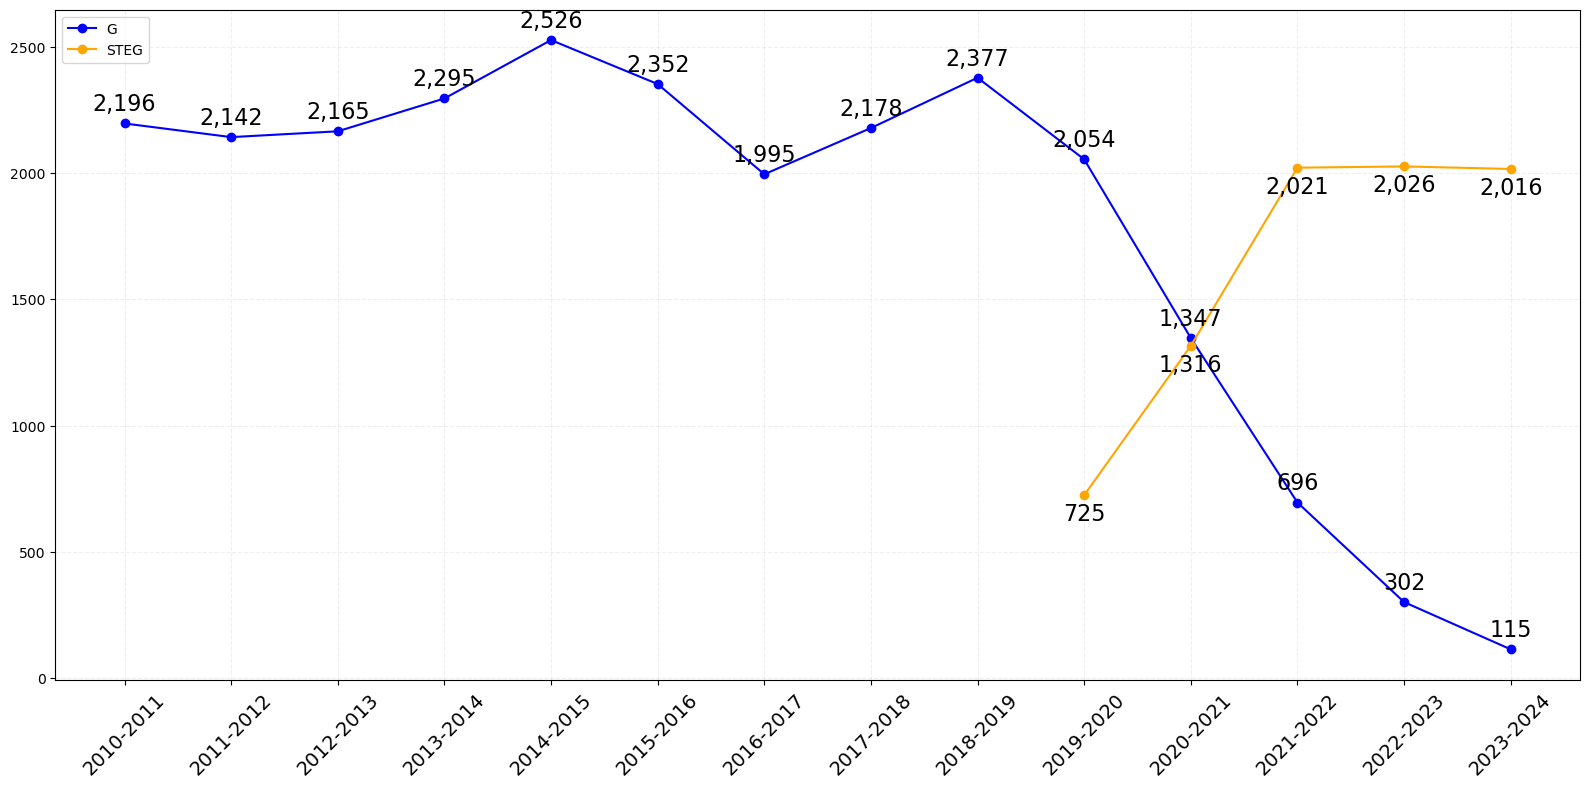
\includegraphics[width=1\textwidth]{figure/Inscrits_ucad_STEG.png}
\label{fig:inscrits_ucad_steg}
\end{figure}

La figure (Figure~\ref{fig:inscrits_ucad_steg}) illustre l'évolution des inscriptions à l'Université Cheikh Anta Diop (UCAD) pour les bacheliers issus des séries G et STEG, sur la période 2010-2011 à 2023-2024.

Jusqu'à l'année universitaire 2018-2019, seule la série G est représentée à l'UCAD, avec un nombre d'inscrits fluctuant autour de 2 000 à 2 500. Un pic est observé en 2014-2015 avec 2 526 inscrits. 
À partir de 2019-2020, la série STEG fait son apparition, avec 725 inscrits, marquant le début de la transition. Simultanément, les effectifs de la série G commencent à décliner fortement, passant de 2 054 en 2019-2020 à seulement 115 en 2023-2024. 
Ce déclin correspond à la suppression progressive de la série G au profit de la série STEG dans le système du baccalauréat.

Le croisement des courbes est particulièrement visible en 2020-2021, où le nombre d'inscrits en STEG (1 347) dépasse celui de la série G (1 316). 
Cette tendance se confirme les années suivantes, la série STEG affichant des effectifs croissants (2 021 en 2021-2022, 2 026 en 2022-2023, et 2 016 en 2023-2024), tandis que la série G continue sa chute. 
La série STEG maintient ainsi un volume d'inscriptions à l'UCAD comparable à celui que la série G connaissait avant sa suppression, démontrant une transition quantitativement réussie au niveau de l'entrée à l'université. 
Ce transfert des effectifs de la série G vers la série STEG à l'UCAD est un indicateur de l'efficacité de la réforme du baccalauréat dans l'orientation des étudiants vers la nouvelle filière.

\newpage
\subsection{Les inscrits des séries Arables et Franco-Arabes}

\subsubsection{Série LA et LAR}

\begin{figure}[ht]
\centering
\caption{Évolution des inscriptions à l'UCAD pour les séries LA et LAR}
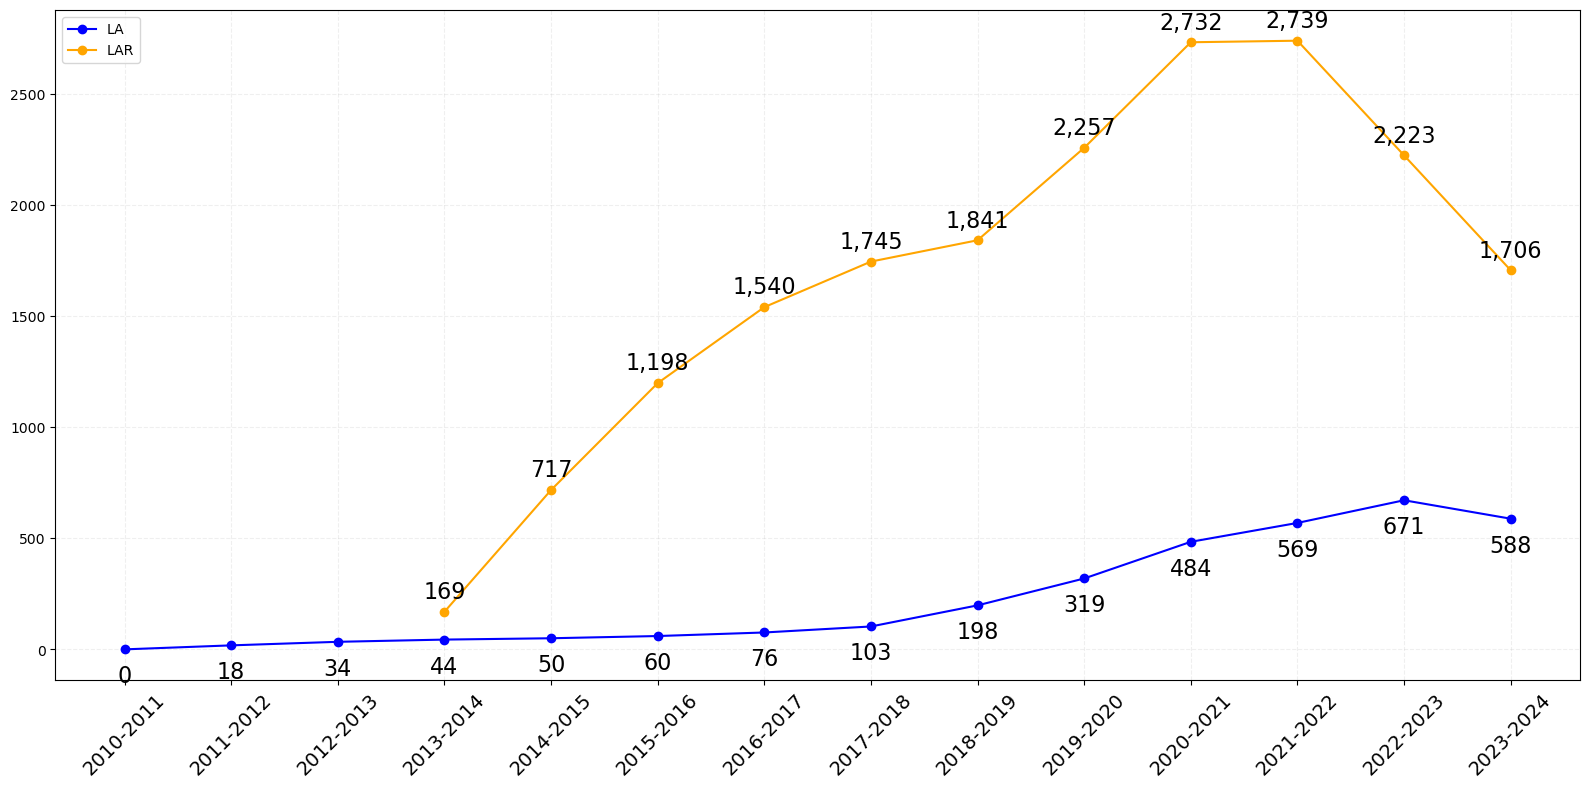
\includegraphics[width=1\textwidth]{figure/Inscrits_ucad_LA_LAR.png}
\label{fig:inscrits_ucad_la_lar}
\end{figure}

La figure (Figure~\ref{fig:inscrits_ucad_la_lar}) présente l'évolution des inscriptions à l'UCAD pour les bacheliers issus des séries Littératures Arabes (LA) et Littératures et Civilisations Arabes (L-AR) de 2010-2011 à 2023-2024.

La série LA, bien que présente depuis 2010-2011, a enregistré un nombre très faible d'inscrits à l'UCAD jusqu'en 2013-2014, oscillant entre 0 et 44. 
À partir de 2014-2015, le nombre d'inscrits en LA connaît une croissance progressive, passant de 50 à 671 en 2022-2023, avant de redescendre légèrement à 588 en 2023-2024.

La série L-AR, introduite à l'UCAD à partir de 2013-2014, a connu une croissance beaucoup plus rapide et significative. Elle débute avec 169 inscrits en 2013-2014 et grimpe rapidement pour atteindre un pic de 2 739 inscrits en 2021-2022. 
Bien qu'une légère diminution soit observée les années suivantes, avec 2 223 inscrits en 2022-2023 et 1 706 en 2023-2024, la série L-AR maintient un volume d'inscriptions considérablement plus élevé que la série LA. 
Ce phénomène s'aligne avec l'observation d'un transfert progressif des effectifs vers la série L-AR au niveau du baccalauréat lui-même, la série L-AR ayant été mise en place pour mieux encadrer et répondre à la demande sociale des filières arabes et franco-arabes. 

% En conclusion, la série L-AR a réussi à s'imposer comme la filière majeure pour les étudiants en études arabes à l'UCAD, absorbant une grande partie des effectifs et démontrant l'impact des réformes du baccalauréat sur l'orientation universitaire.

\newpage
\subsubsection{Série S2A et S1A}

\begin{figure}[ht]
\centering
\caption{Évolution des inscriptions à l'UCAD pour les séries S2A et S1A}
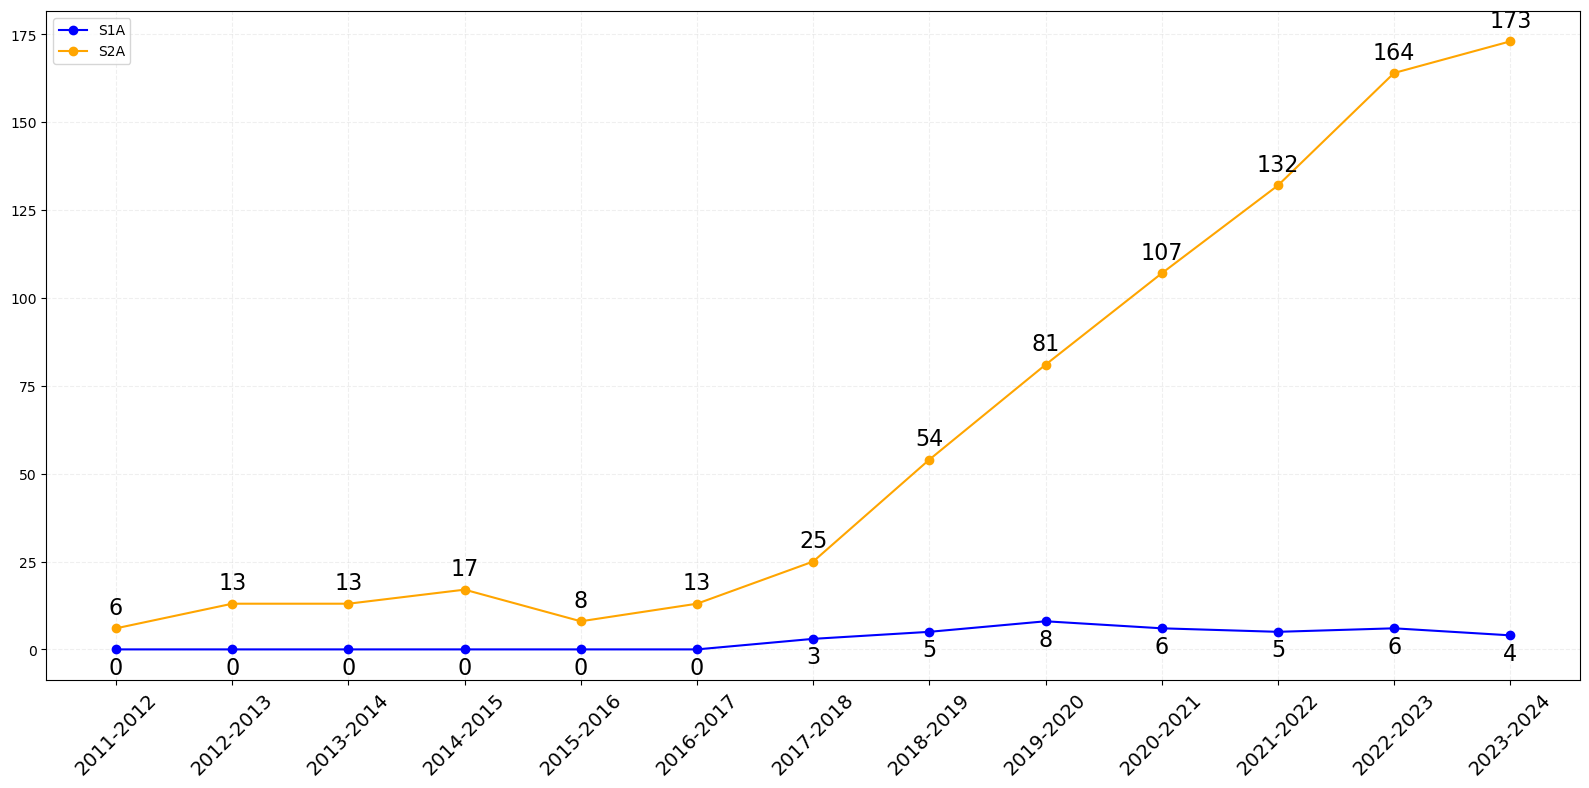
\includegraphics[width=1\textwidth]{figure/Inscrits_ucad_SA.png}
\label{fig:inscrits_ucad_sa}
\end{figure}

La figure (Figure~\ref{fig:inscrits_ucad_sa}) retrace l'évolution des inscriptions à l'UCAD pour les bacheliers des séries Sciences fondamentales (S1A) et Sciences appliquées (S2A) entre 2011-2012 et 2023-2024.

La série S1A, bien que présente, affiche un nombre d'inscrits extrêmement faible à l'UCAD tout au long de la période. Les effectifs oscillent entre 0 et 8 (atteint en 2019-2020), avec seulement 4 inscrits en 2023-2024. 
Cette quasi-absence d'inscriptions à l'université confirme le caractère très marginal de cette filière, qui déjà au niveau du baccalauréat, n'attire qu'un nombre dérisoire de candidats. 
Cela suggère que la série S1A ne débouche que sur très peu d'orientations universitaires à l'UCAD.

En revanche, la série S2A présente une dynamique d'inscriptions beaucoup plus significative. Après des débuts modestes entre 6 et 17 inscrits de 2011-2012 à 2015-2016, le nombre d'étudiants en S2A à l'UCAD connaît une croissance exponentielle. 
On passe de 25 inscrits en 2016-2017 à 107 en 2020-2021, pour atteindre un pic de 173 inscrits en 2023-2024. Cette forte augmentation des inscriptions en S2A à l'UCAD reflète une reconnaissance croissante de cette filière scientifique parmi les bacheliers arabes et franco-arabes, leur offrant des perspectives universitaires concrètes.

En somme, l'analyse des inscriptions à l'UCAD confirme les dynamiques observées au niveau du baccalauréat : la série S1A reste une filière confidentielle, tandis que la S2A gagne en importance et en attractivité pour les études supérieures, offrant ainsi une voie viable aux bacheliers issus de l'enseignement scientifique arabe et franco-arabe.

\newpage
\section{Répartition des Inscrits par Établissement et Département}

\subsection{Série STEG et G}

% \subsubsection{Série G}

\textbf{Répartition par Établissements}

\begin{figure}[ht]
\centering
\caption{Top 5 des établissements avec le plus d'inscrits (G, 2018-2019)}
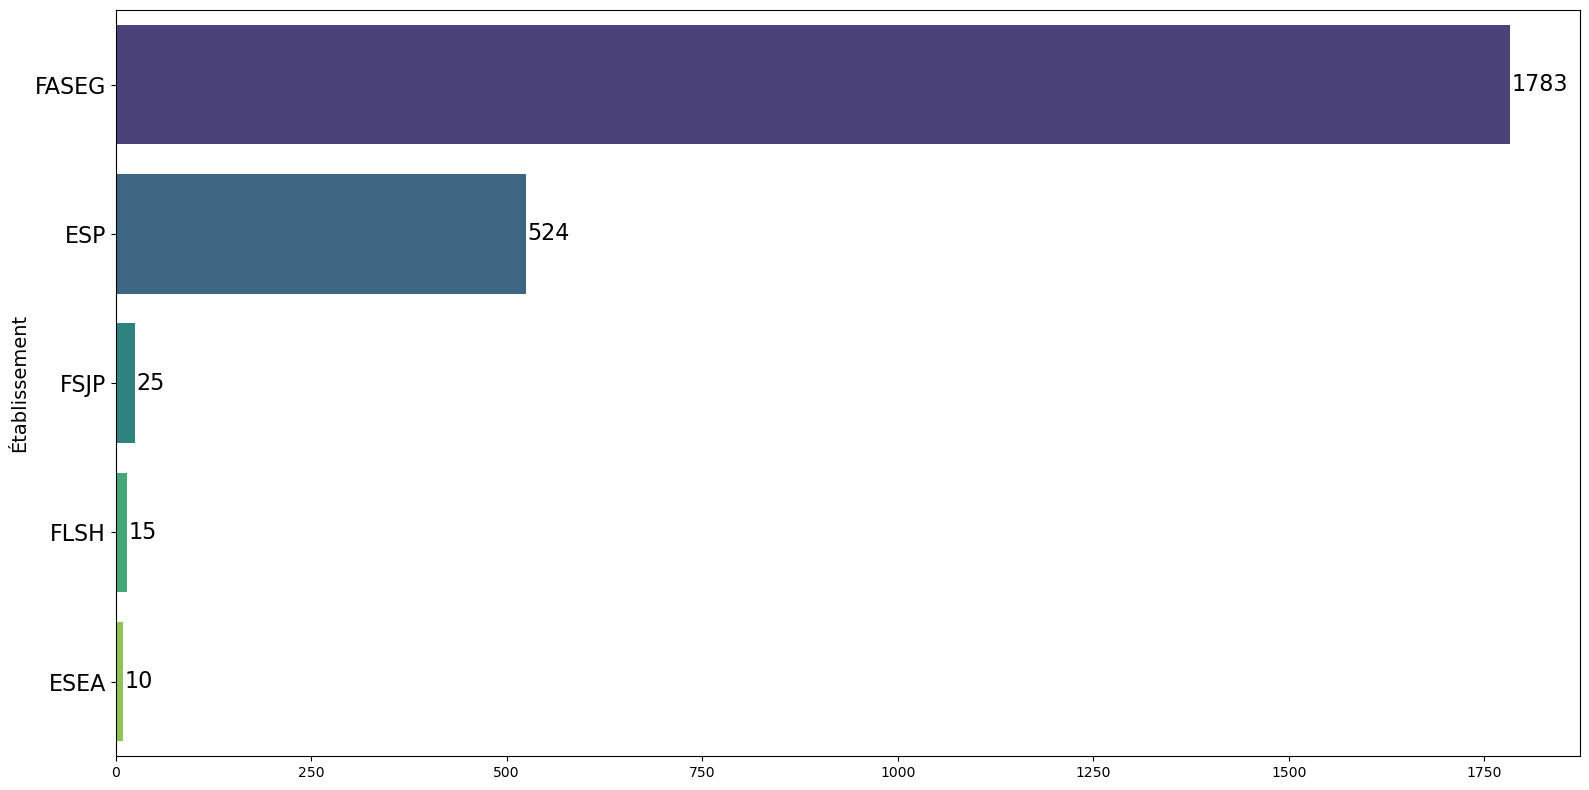
\includegraphics[width=0.8\textwidth]{figure/etab_G_2019.png}
\label{fig:etab_g_2019}
\end{figure}

La Figure \ref{fig:etab_g_2019} présente la répartition des inscriptions des bacheliers G au sein des établissements de l'UCAD pour l'année universitaire 2018-2019.

Avant la réforme complète, en 2019, la Faculté des Sciences Économiques et de Gestion (FASEG) était déjà l'établissement accueillant la majorité des bacheliers de la série G, avec 1783 inscrits, suivie par l'École Supérieure Polytechnique (ESP) avec 524 inscrits. 

% \newpage
\begin{figure}[ht]
\centering
\caption{Top 5 des établissements avec le plus d'inscrits (STEG, 2023-2024)}
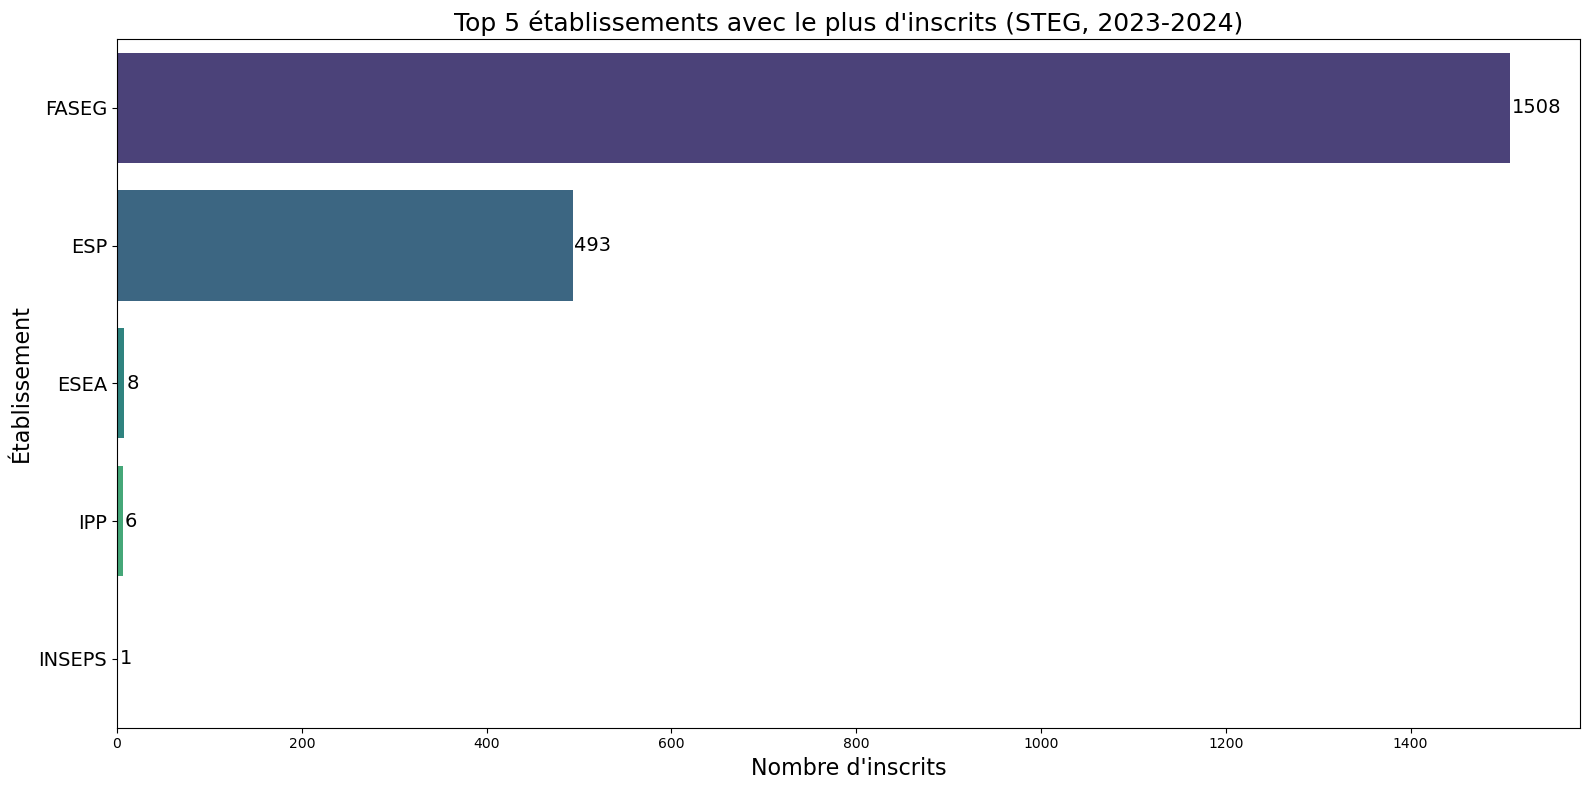
\includegraphics[width=0.8\textwidth]{figure/etab_STEG_2024.png}
\label{fig:etab_steg_2024}
\end{figure}

La Figure \ref{fig:etab_steg_2024} présente la répartition des inscriptions des bacheliers STEG au sein des établissements de l'UCAD pour l'année universitaire 2023-2024.

Pour l'année universitaire 2023-2024, après la transformation de la série G en STEG, la FASEG continue de dominer très largement les inscriptions des bacheliers STEG à l'UCAD, accueillant 1508 étudiants. 
L'École Supérieure Polytechnique (ESP) maintient sa deuxième position avec 493 inscrits. Ces chiffres confirment que, malgré le changement de dénomination et d'orientation pédagogique, la FASEG demeure la principale destination pour les bacheliers de cette filière, en raison de la nature économique et de gestion de la série STEG. 

% \newpage
\textbf{Répartition par Départements}

\begin{figure}[ht]
\centering
\caption{Top 5 des départements avec le plus d'inscrits (G, 2018-2019)}
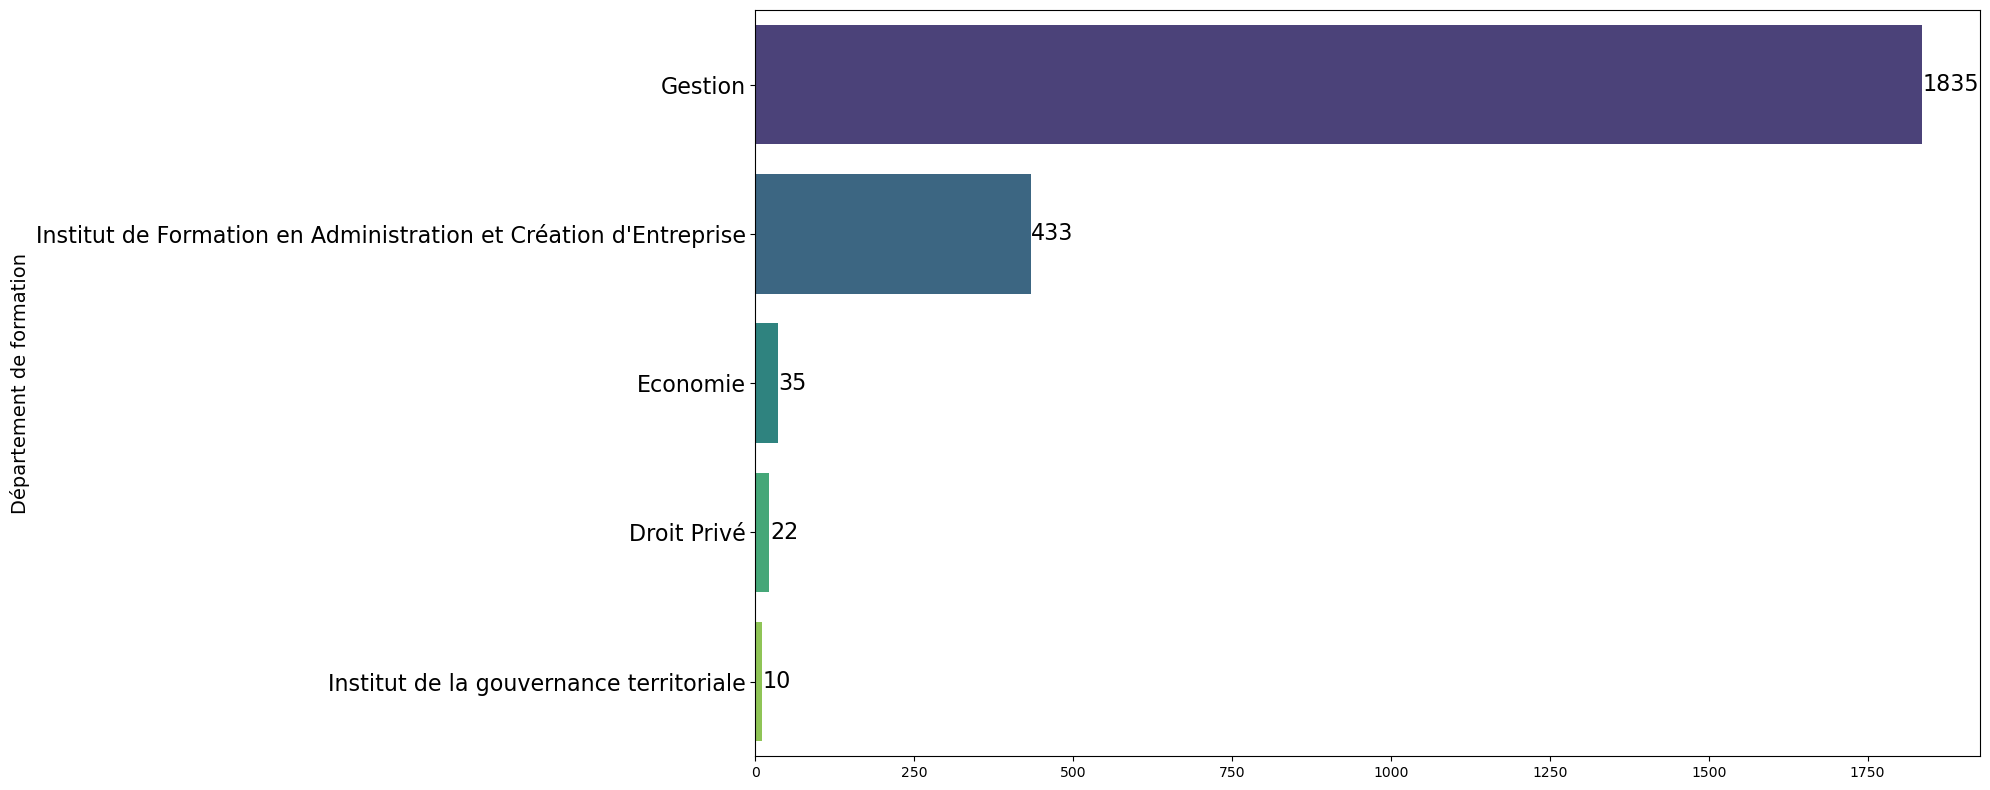
\includegraphics[width=0.8\textwidth]{figure/dep_G_2019.png}
\label{fig:dep_g_2019}
\end{figure}

La Figure \ref{fig:dep_g_2019} illustre la répartition des inscrits G par département de formation à l'UCAD pour l'année universitaire 2018-2019.

En 2019, le département de Gestion concentrait la grande majorité des inscrits de la série G, avec 1835 étudiants, suivi par l'Institut de Formation en Administration et Création d'Entreprise avec 433 inscrits. Le département d'Économie comptait 35 inscrits.

% Le département de Gestion se positionne très largement en tête, avec 1 623 inscrits. Cette dominance est logique et attendue, étant donné l'orientation principale de la série G vers les sciences et techniques de gestion. 

\begin{figure}[ht]
\centering
\caption{Top 5 des départements avec le plus d'inscrits (STEG, 2023-2024)}
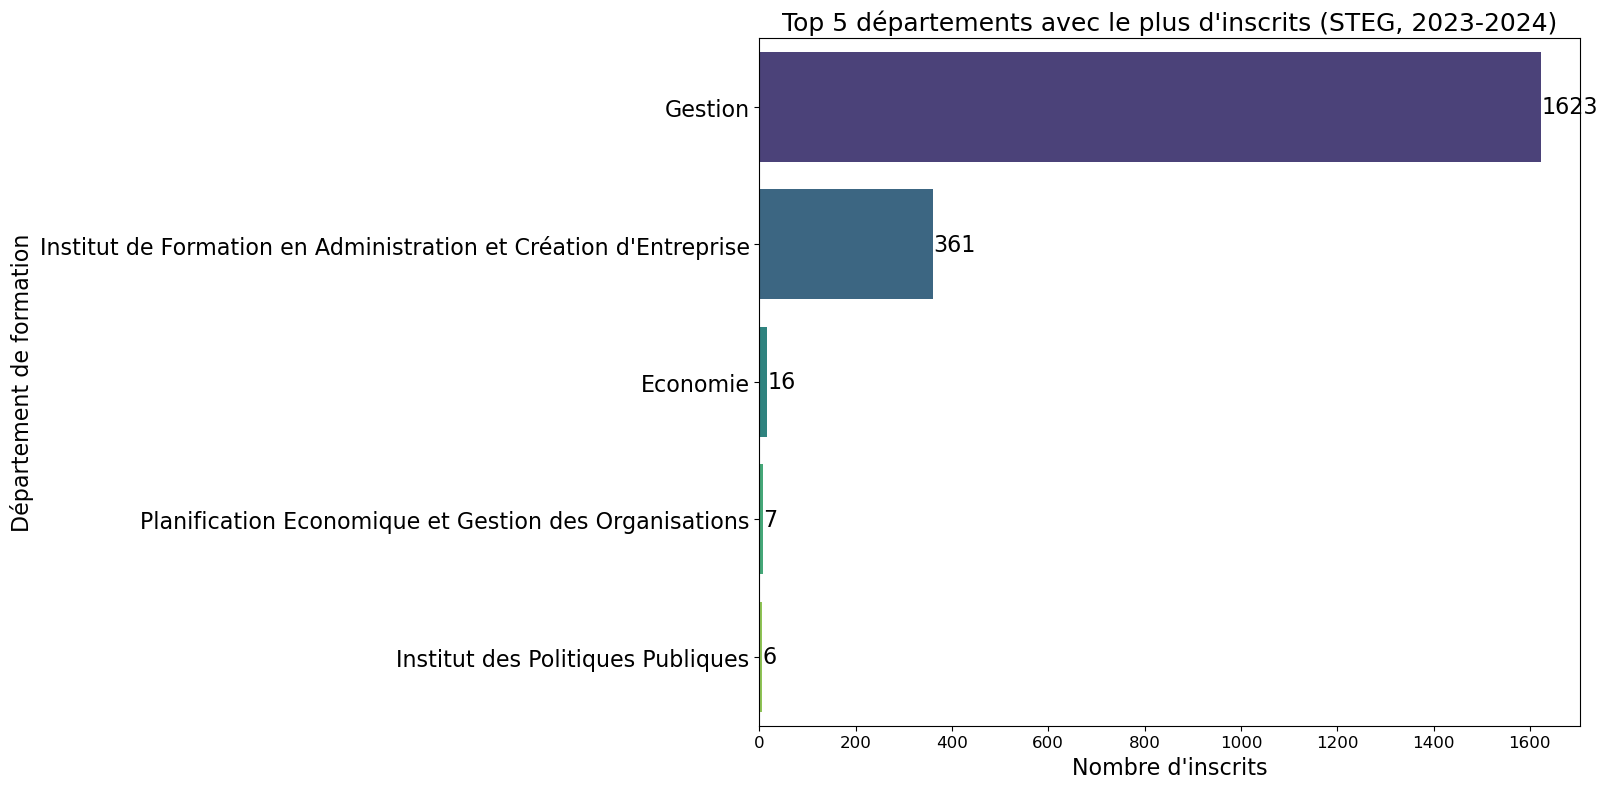
\includegraphics[width=0.8\textwidth]{figure/dep_STEG_2024.png}
\label{fig:dep_steg_2024}
\end{figure}

La Figure \ref{fig:dep_steg_2024} illustre la répartition des inscrits STEG par département de formation à l'UCAD pour l'année universitaire 2023-2024.

Pour l'année universitaire 2023-2024, le département de Gestion conserve sa position dominante pour les inscrits de la série STEG, avec 1623 inscrits. L'Institut de Formation en Administration et Création d'Entreprise suit avec 361 inscrits. 
Le département d'Économie compte 16 inscrits. Cette répartition des inscrits par département, avant et après la réforme, confirme la forte vocation de cette série pour les études en gestion, avec un intérêt secondaire pour l'entrepreneuriat, et une présence marginale dans les autres branches de l'économie. 

% \newpage
\subsection{Série Arabes et Franco-Arabes}

\subsubsection{Série LA}

\textbf{Établissements}

\begin{figure}[ht]
\centering
\caption{Top 5 des établissements avec le plus d'inscrits (LA, 2023-2024)}
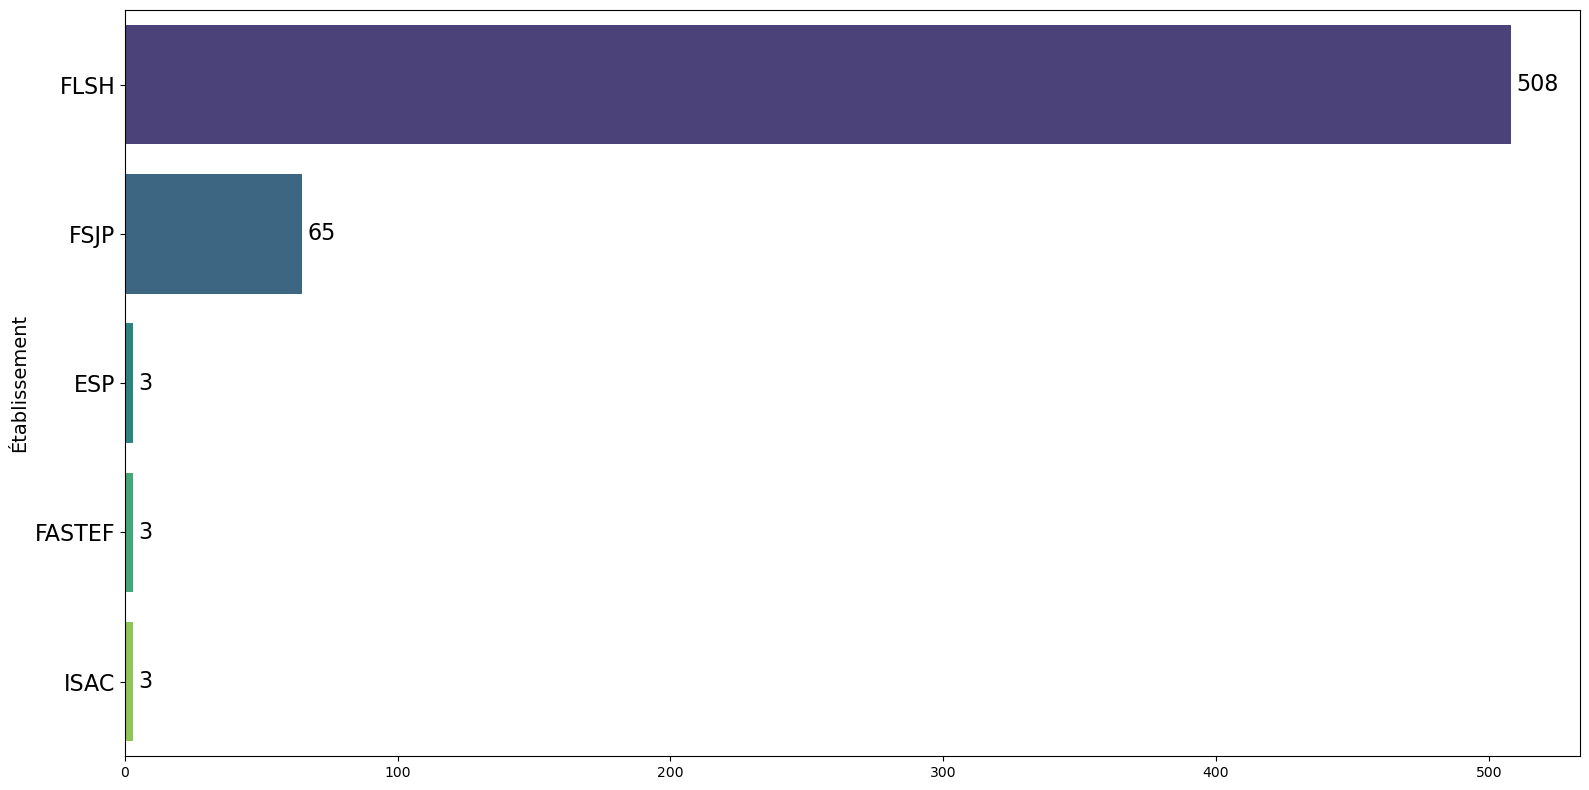
\includegraphics[width=0.8\textwidth]{figure/etab_LA_2024.png}
\label{fig:etab_la_2024}
\end{figure}

La Figure \ref{fig:etab_la_2024} montre la répartition des inscrits de la série LA par établissement à l'UCAD pour l'année universitaire 2023-2024.

La Faculté des Lettres et Sciences Humaines (FLSH) est l'établissement qui accueille de loin le plus grand nombre de bacheliers LA, avec 508 inscrits. 
Cette prédominance est entièrement cohérente avec la nature littéraire de la série LA, la FLSH étant traditionnellement le pôle d'excellence pour les études de lettres, de langues et de civilisations.

La Faculté des Sciences Juridiques et Politiques (FSJP) arrive en deuxième position avec 65 inscrits. Bien que significativement moins importante que la FLSH, la présence de bacheliers LA dans cette faculté peut s'expliquer par un intérêt pour le droit islamique.

\newpage
\textbf{Départements}

\begin{figure}[ht]
\centering
\caption{Top 5 des départements avec le plus d'inscrits (LA, 2023-2024)}
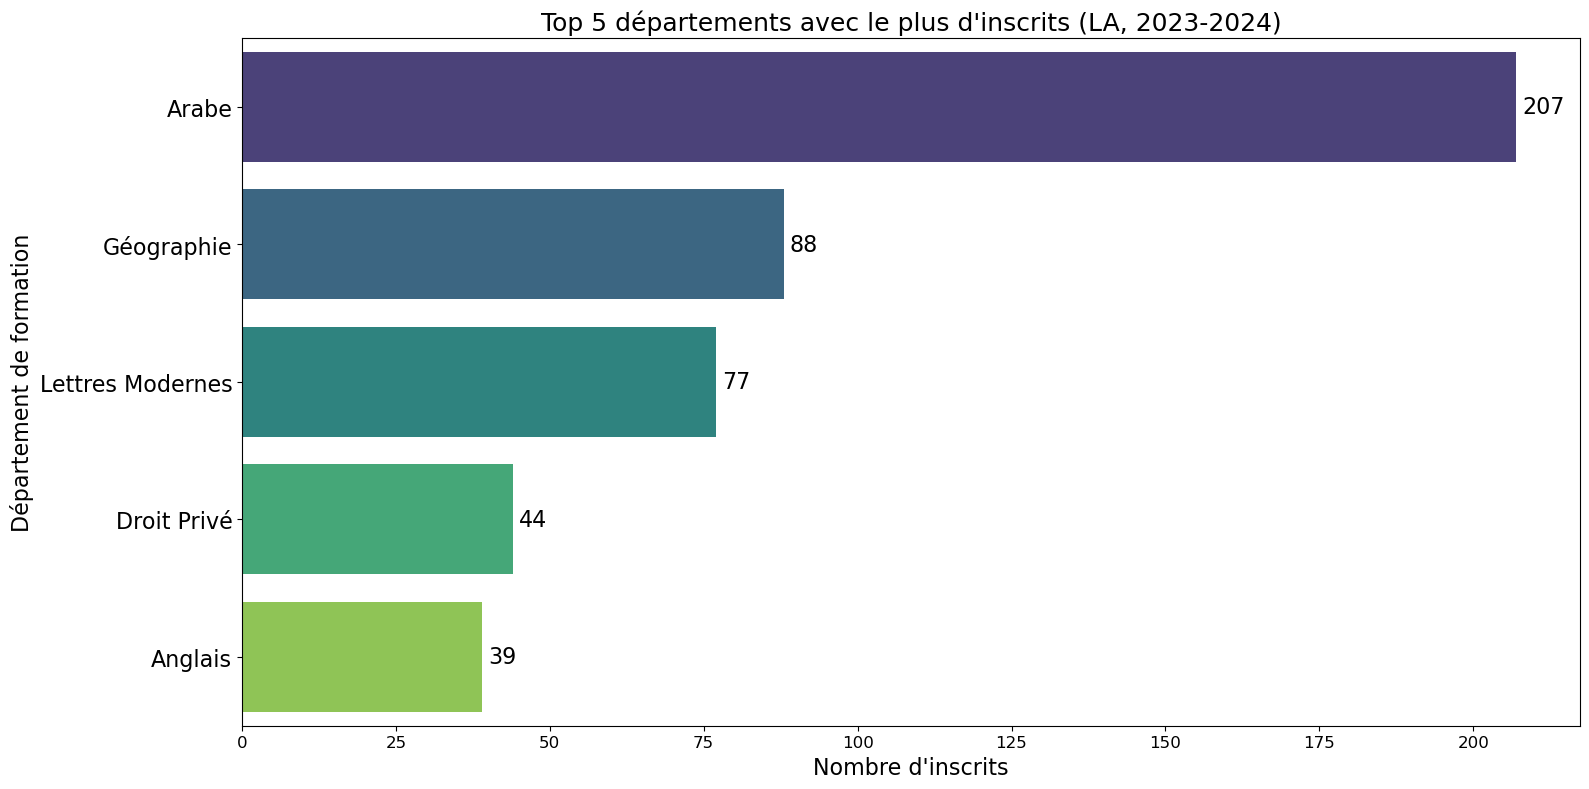
\includegraphics[width=0.8\textwidth]{figure/dep_LA_2024.png}
\label{fig:dep_la_2024}
\end{figure}

La Figure \ref{fig:dep_la_2024} présente la répartition des inscrits de la série LA par département de formation à l'UCAD pour l'année universitaire 2023-2024.

Le département d'Arabe domine avec 207 bacheliers LA, ce qui est attendu pour cette série littéraire axée sur la langue arabe
Cependant, d’autres départements comme la Géographie (88), les Lettres Modernes (77), le Droit Privé (44) et l’Anglais (39) attirent aussi des bacheliers LA

Cette dispersion s’explique par le caractère franco-arabe de la série LA, qui offre plus de flexibilité que la série LAR, permettant aux étudiants de s’orienter vers un éventail plus large de filières en sciences humaines.
% \newpage
\subsubsection{Série LAR}

\textbf{Établissements}

\begin{figure}[ht]
\centering
\caption{Top 5 des établissements avec le plus d'inscrits (LAR, 2023-2024)}
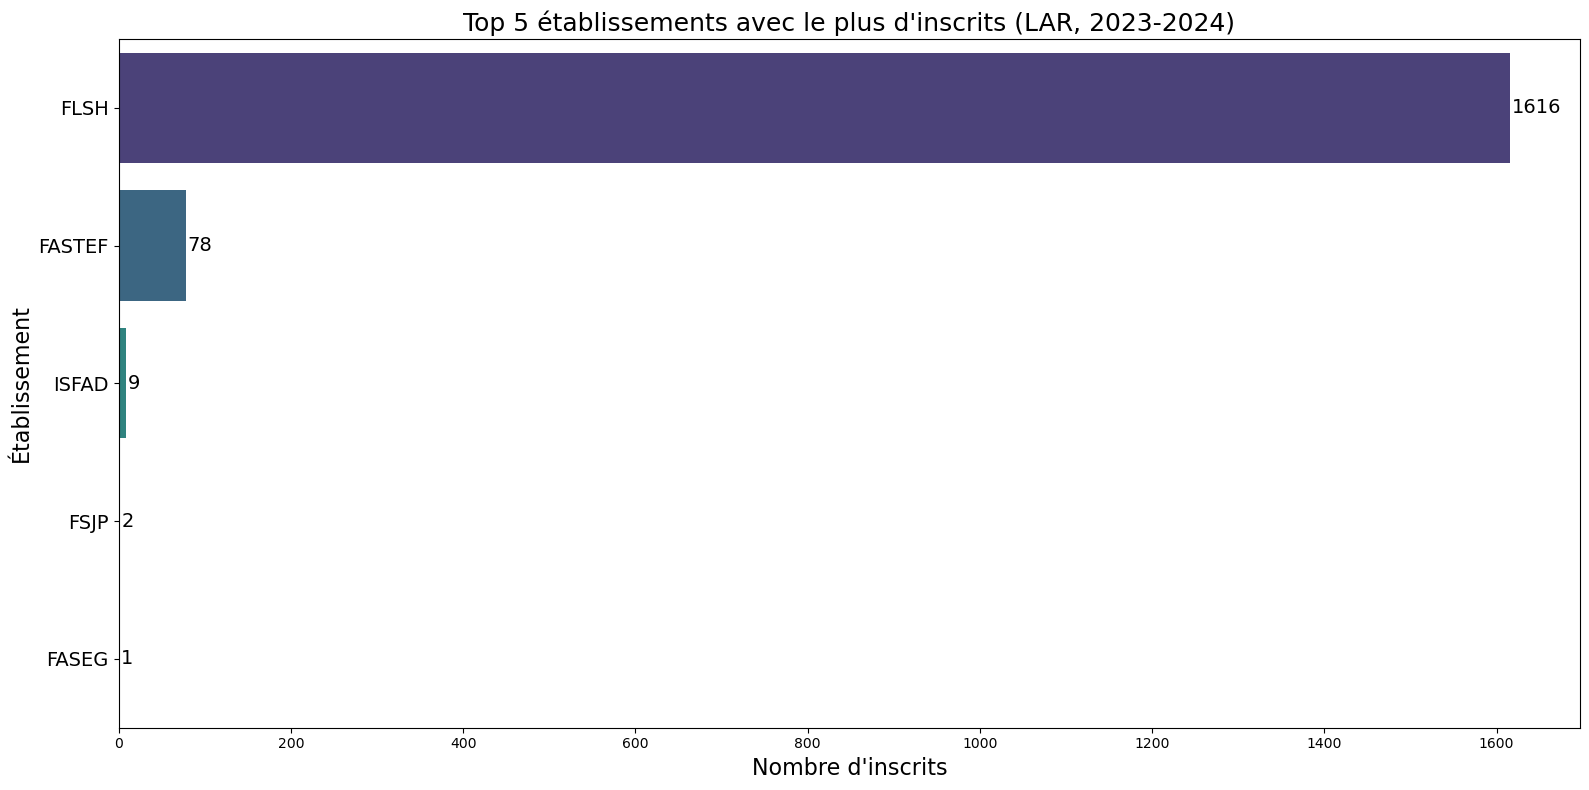
\includegraphics[width=0.8\textwidth]{figure/etab_LAR_2024.png}
\label{fig:etab_lar_2024}
\end{figure}

La Figure \ref{fig:etab_lar_2024} illustre la répartition des inscrits de la série LAR par établissement à l'UCAD pour l'année universitaire 2023-2024.

Comme pour la série LA, la Faculté des Lettres et Sciences Humaines (FLSH) est l’établissement le plus plébiscité par les bacheliers LAR, avec un total massif de 1 616 inscrits. 
Cette écrasante majorité confirme le rôle central de la FLSH dans la formation en langue, littérature et civilisation arabes, faisant de cette faculté la destination naturelle et presque exclusive des bacheliers issus de cette série.

En deuxième position, la FASTEF accueille 78 inscrits. Cette orientation s'explique par les débouchés dans l’enseignement, en particulier pour les matières liées à la langue arabe ou à l’éducation islamique, domaines en cohérence avec la formation reçue dans la série LAR.

À l’inverse, la Faculté des Sciences Juridiques et Politiques (FSJP) ne compte que 2 inscrits LAR, contre 65 pour la série LA. 
Cette faible représentation s’explique très probablement par une contrainte linguistique importante : 
les enseignements à la FSJP se déroulant majoritairement en français, les bacheliers LAR, dont la formation est exclusivement en arabe, peuvent être freinés dans leur orientation vers des filières francophones, contrairement aux bacheliers LA disposant d’une double compétence linguistique.

\textbf{Départements}

\begin{figure}[ht]
\centering
\caption{Top 5 des départements avec le plus d'inscrits (LAR, 2023-2024)}
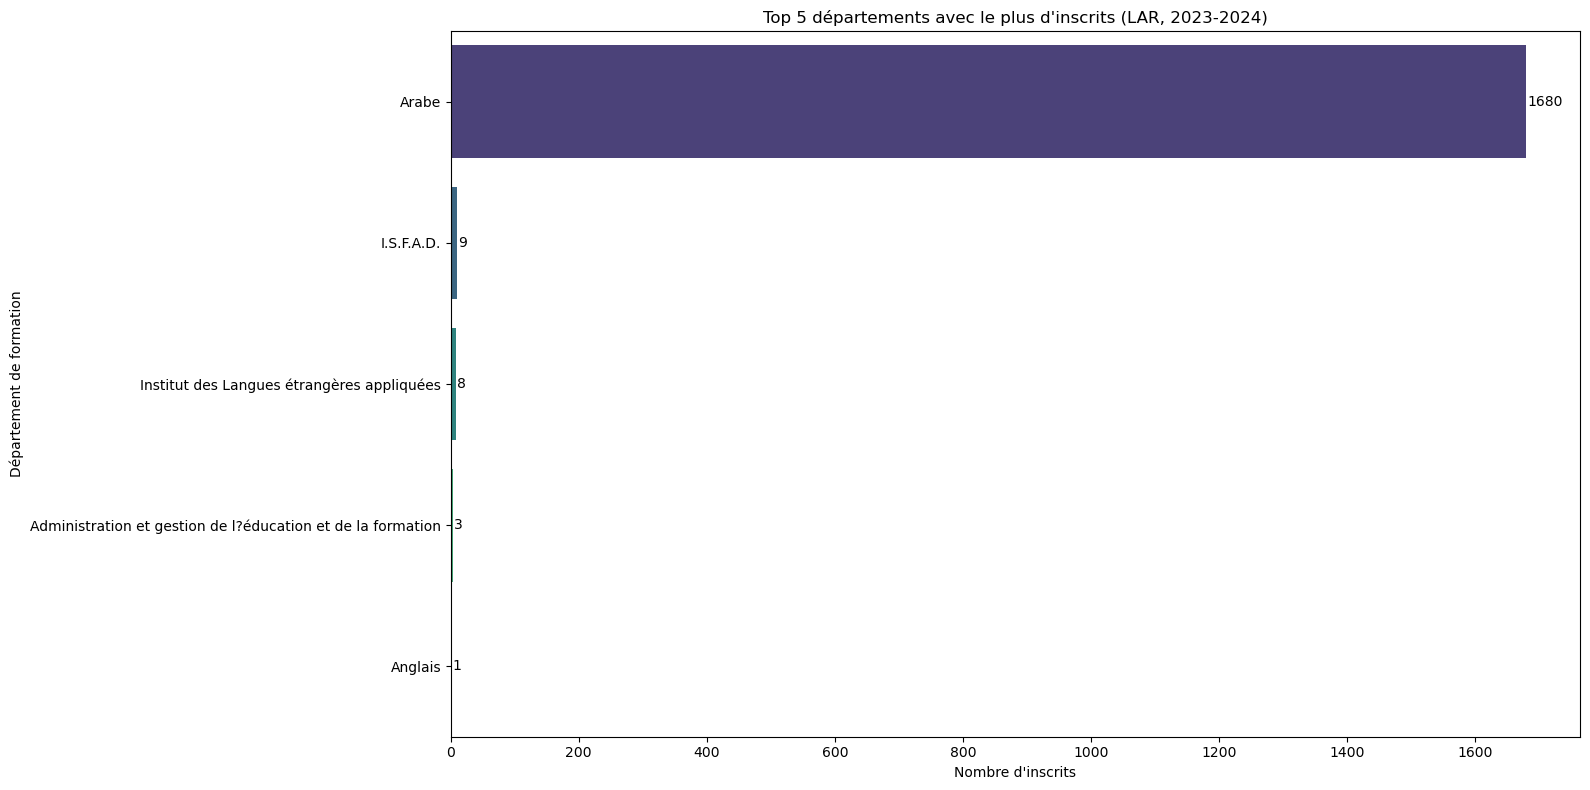
\includegraphics[width=0.8\textwidth]{figure/dep_LAR_2024.png}
\label{fig:dep_lar_2024}
\end{figure}

% La Figure \ref{fig:dep_lar_2024} détaille la répartition des inscrits de la série LAR par département de formation à l'UCAD pour l'année universitaire 2023-2024.

Le département d’Arabe domine de manière écrasante avec 1 680 inscrits, concentrant ainsi presque la totalité des bacheliers LAR. 
Cette prépondérance est tout à fait attendue, la série LAR (Littératures et Civilisations Arabes) étant spécifiquement conçue pour préparer les étudiants à des études approfondies en langue, littérature et culture arabes. 
Le département d’Arabe représente donc la destination la plus logique, naturelle et cohérente pour ces profils.

En conclusion, l’orientation des bacheliers LAR est quasiment exclusive vers le département d’Arabe, traduisant une spécialisation universitaire marquée, en parfaite continuité avec leur formation secondaire.

\subsubsection{Série S2A}

\textbf{Établissements}

\begin{figure}[ht]
\centering
\caption{Top 5 des établissements avec le plus d'inscrits (S2A, 2023-2024)}
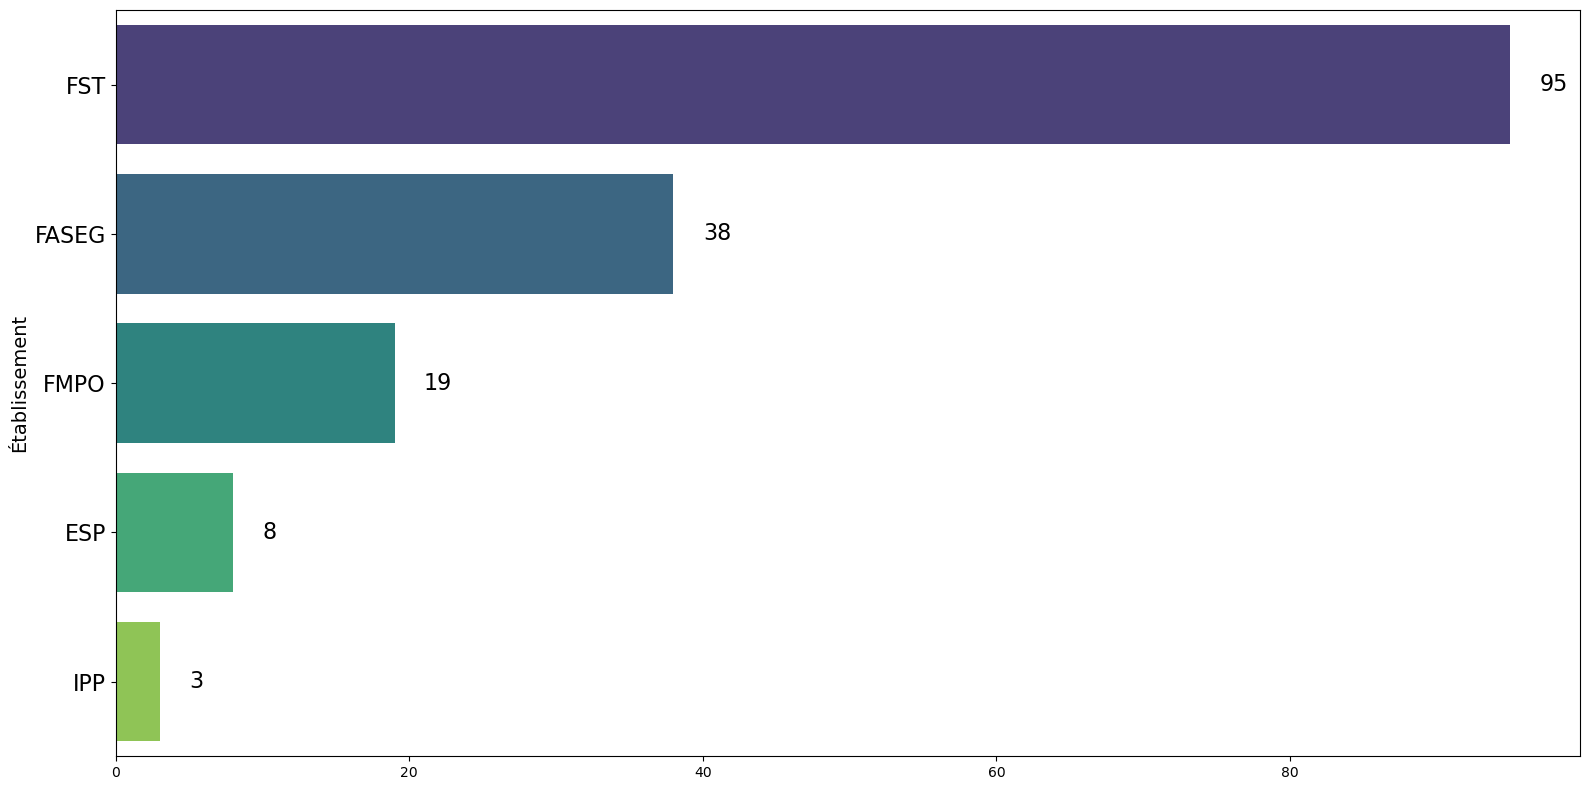
\includegraphics[width=0.8\textwidth]{figure/etab_S2A_2024.png}
\label{fig:etab_s2a_2024}
\end{figure}

La Figure \ref{fig:etab_s2a_2024} présente la répartition des inscrits de la série S2A par établissement à l'UCAD pour l'année universitaire 2023-2024.

La FST domine avec 95 inscrits, reflet de l’orientation scientifique de la série S2A. 
D’autres établissements accueillent aussi ces étudiants, notamment la FASEG (38), la FMPO (19), ainsi que plus modestement l’ESP et l’IPP. Cette répartition illustre la polyvalence et l’adaptabilité des diplômés S2A, qui s’intègrent dans des filières variées allant des sciences à l’économie, la santé ou l’ingénierie.

\textbf{Départements}

\begin{figure}[ht]
\centering
\caption{Top 5 des départements avec le plus d'inscrits (S2A, 2023-2024)}
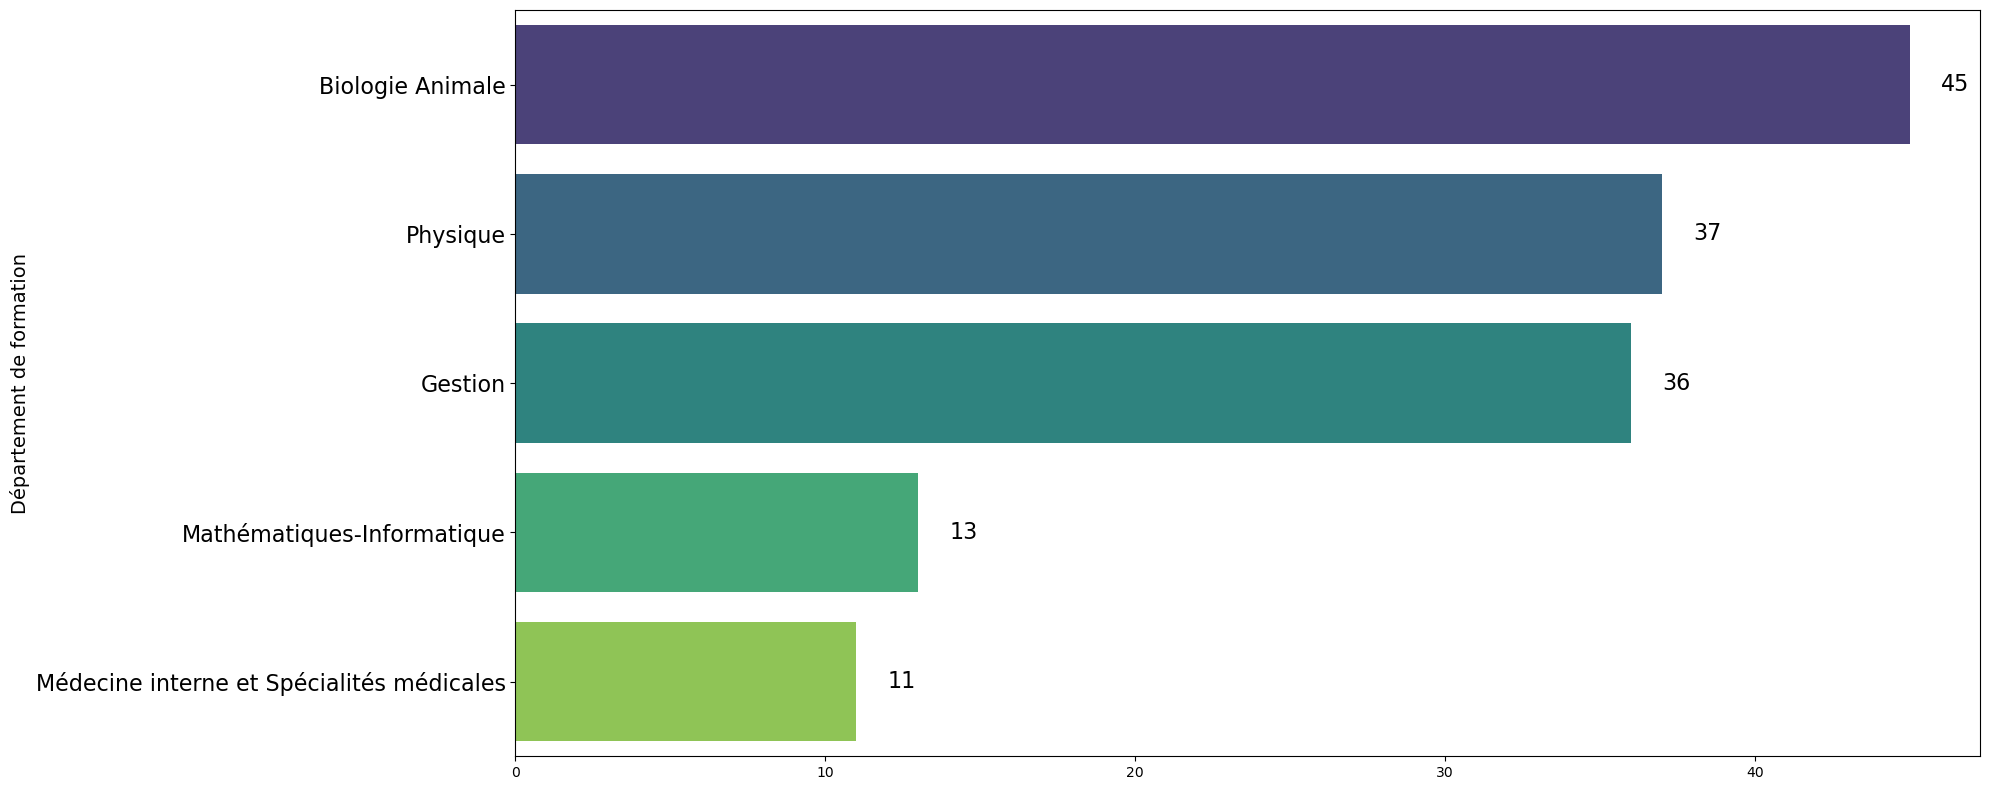
\includegraphics[width=0.8\textwidth]{figure/dep_S2A_2024.png}
\label{fig:dep_s2a_2024}
\end{figure}

La Figure \ref{fig:dep_s2a_2024} détaille la répartition des inscrits de la série S2A par département de formation à l'UCAD pour l'année universitaire 2023-2024.

Le département de Biologie Animale accueille le plus grand nombre de bacheliers S2A (45 inscrits), reflétant leur intérêt pour les sciences du vivant. 
Les départements de Mathématiques-Informatique (13) et de Médecine (11) enregistrent des effectifs plus modestes, montrant une ouverture vers des filières techniques et médicales. 
Cette diversité souligne la capacité des bacheliers S2A à s’intégrer dans des parcours variés grâce à leur formation polyvalente.

\newpage
\subsubsection{Série S1A}

\textbf{Établissements}

\begin{figure}[ht]
\centering
\caption{Top 5 des établissements avec le plus d'inscrits (S1A, 2023-2024)}
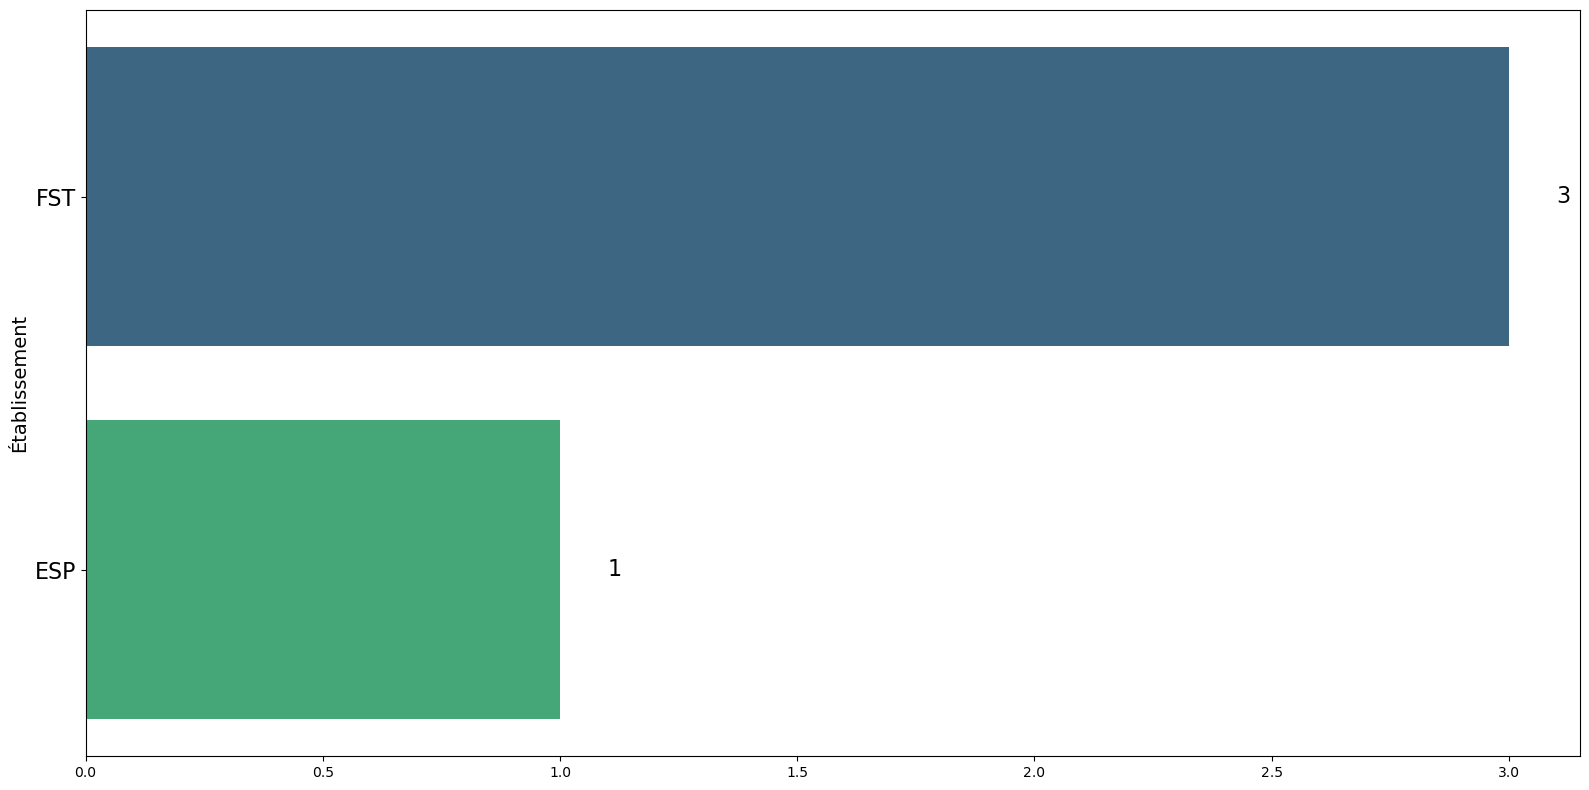
\includegraphics[width=0.8\textwidth]{figure/etab_S1A_2024.png}
\label{fig:etab_s1a_2024}
\end{figure}

La Figure \ref{fig:etab_s1a_2024} présente la répartition des inscrits de la série S1A par établissement à l'UCAD pour l'année universitaire 2023-2024.

La Faculté des Sciences et Technologies (FST) est la principale destination avec 3 inscrits, ce qui correspond à la nature fondamentale de la série S1A. 
L’École Supérieure Polytechnique (ESP) accueille un seul inscrit, reflétant un intérêt marginal pour les formations techniques.

Cependant, le très faible nombre d’inscrits dans ces établissements souligne la rareté de cette série à l’UCAD. 
Ces données limitées ne permettent pas de tirer de conclusions robustes sur les choix d’orientation des bacheliers S1A.

\textbf{Départements}

\begin{figure}[ht]
\centering
\caption{Top 5 des départements avec le plus d'inscrits (S1A, 2023-2024)}
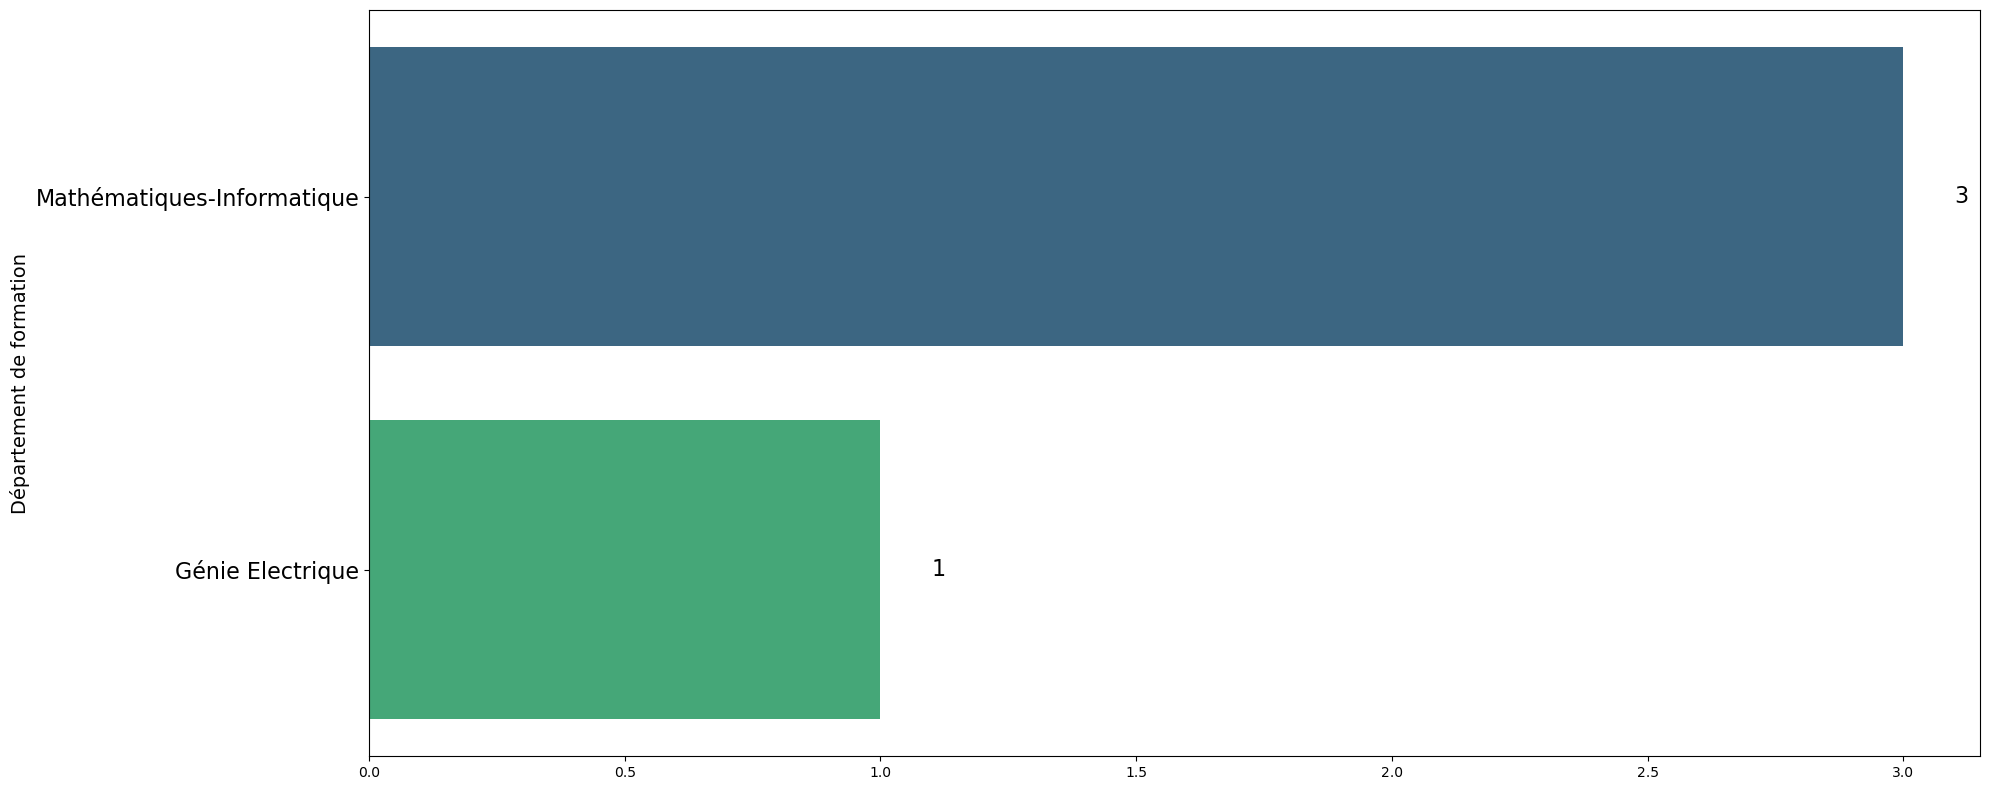
\includegraphics[width=0.8\textwidth]{figure/dep_S1A_2024.png}
\label{fig:dep_s1a_2024}
\end{figure}

\newpage
La Figure \ref{fig:dep_s1a_2024} illustre la répartition des inscrits de la série S1A par département de formation à l'UCAD pour l'année universitaire 2023-2024.

Le département de Mathématiques-Informatique compte 3 inscrits, ce qui correspond bien au profil scientifique fondamental de la série S1A. Le Génie Électrique accueille 1 étudiant, reflétant un intérêt pour des applications techniques. 
Ces effectifs limités confirment la faible présence des bacheliers S1A à l’UCAD, qui restent néanmoins orientés vers des filières scientifiques et d’ingénierie spécialisées.

\newpage
\section{Analyse du parcours universitaire des bacheliers (suivi des cohortes)}

\subsection{Série Arabes et Franco-Arabes}
\subsubsection{cohorte 2018(LA)}

\begin{figure}[ht]
    \centering
    \caption{Graphe suivi de la cohorte 2018 (LA)}
    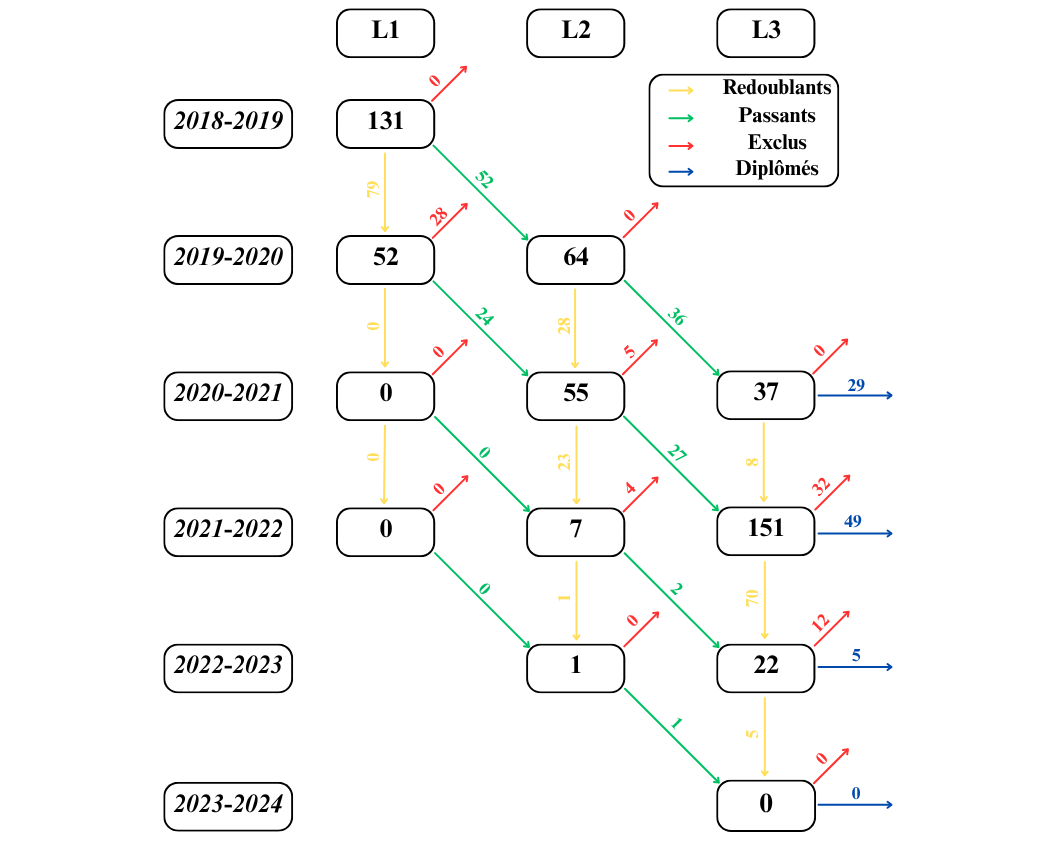
\includegraphics[width=1\textwidth]{figure/LA_2018.png}
\end{figure}

\newpage
\subsubsection{cohorte 2018(LAR)}

\begin{figure}[ht]
    \centering
    \caption{Graphe suivi de la cohorte 2018 (LAR)}
    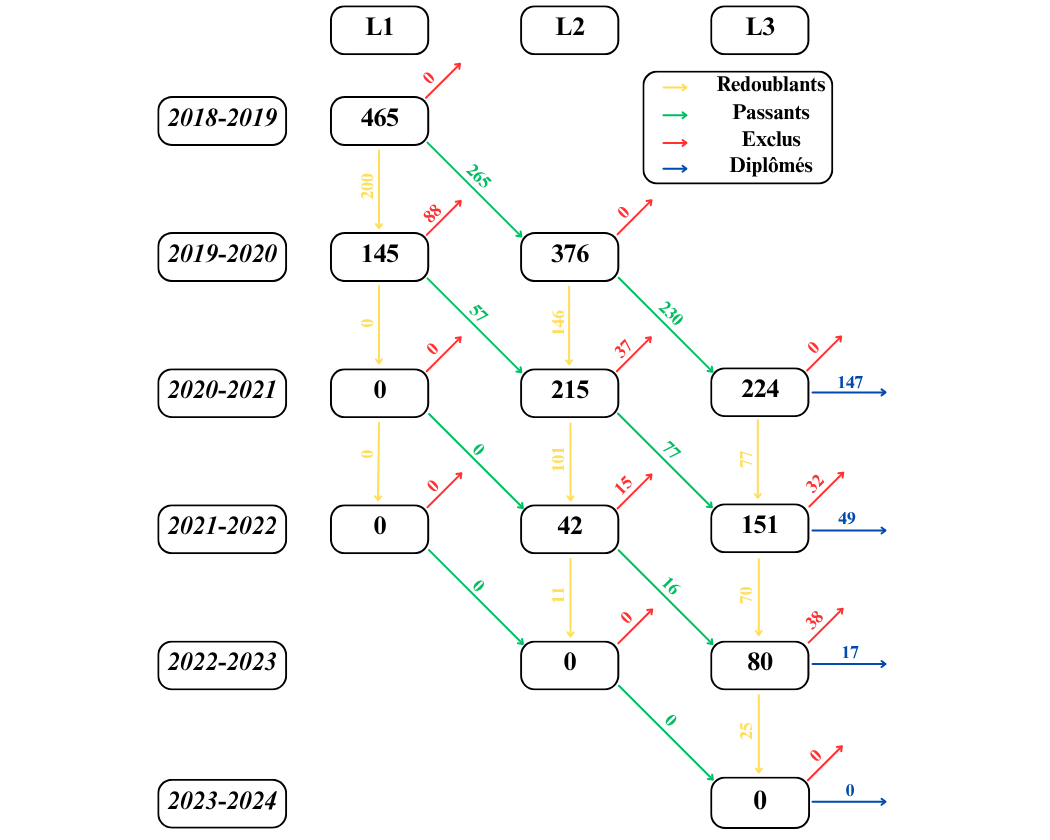
\includegraphics[width=1\textwidth]{figure/LAR_2018.png}
\end{figure}

\newpage
\subsubsection{cohorte 2018(S2A)}

\begin{figure}[ht]
    \centering
    \caption{Graphe suivi de la cohorte 2018 (S2A)}
    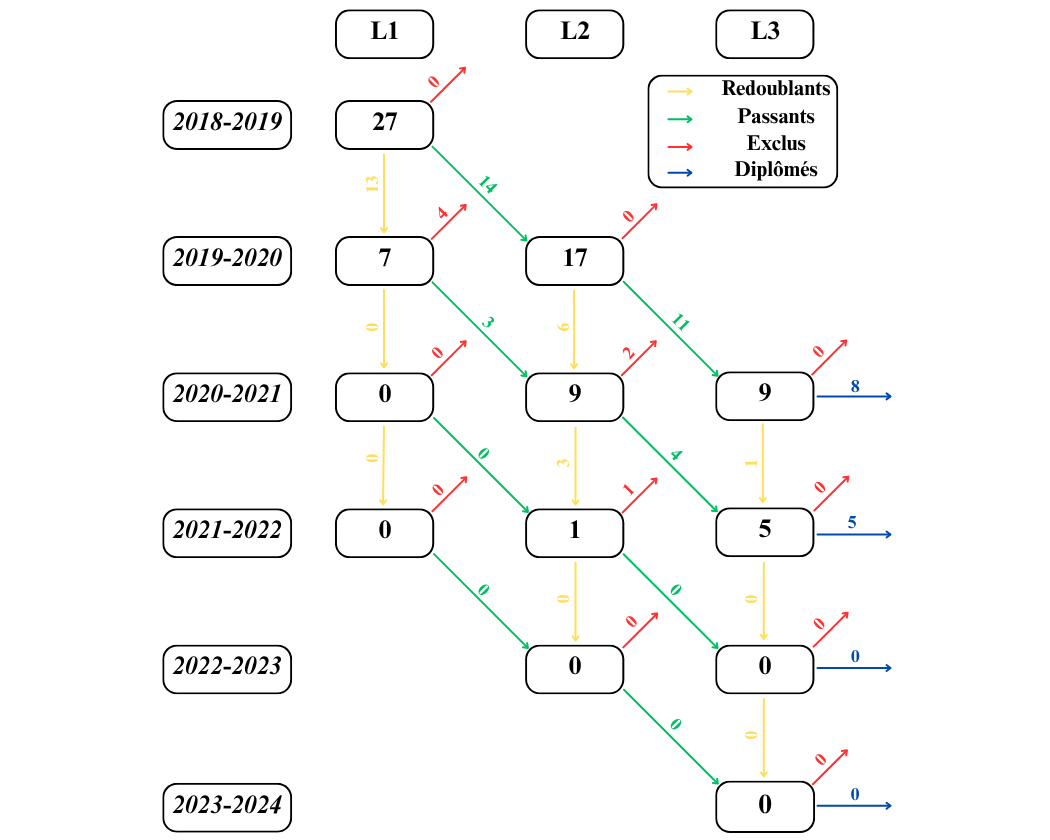
\includegraphics[width=1\textwidth]{figure/S2A_2018.png}
\end{figure}

\newpage
\subsubsection{cohorte 2018(S1A)}

\begin{figure}[ht]
    \centering
    \caption{Graphe suivi de la cohorte 2018 (S1A)}
    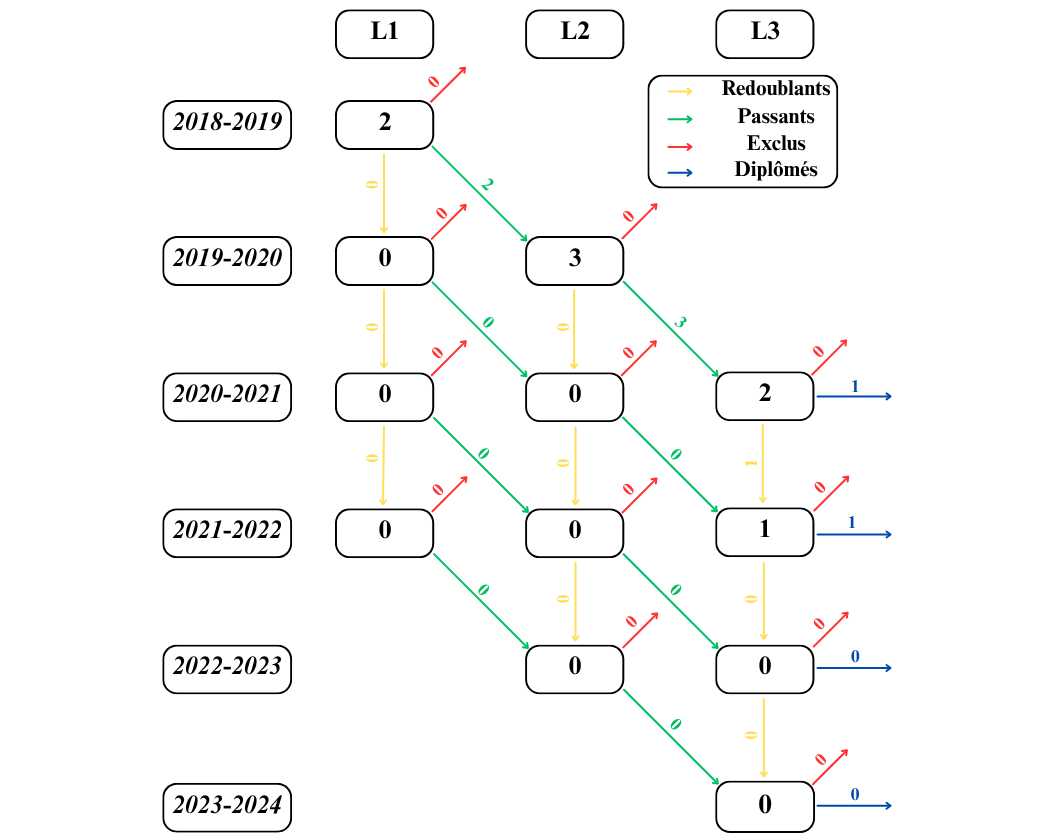
\includegraphics[width=1\textwidth]{figure/S1A_2018.png}
\end{figure}

\newpage
\subsection{Série de reference pour les séries Arabes et Franco-Arabes}

\subsubsection{cohorte 2018(L'1)}

\begin{figure}[ht]
    \centering
    \caption{Graphe suivi de la cohorte 2018 (L'1)}
    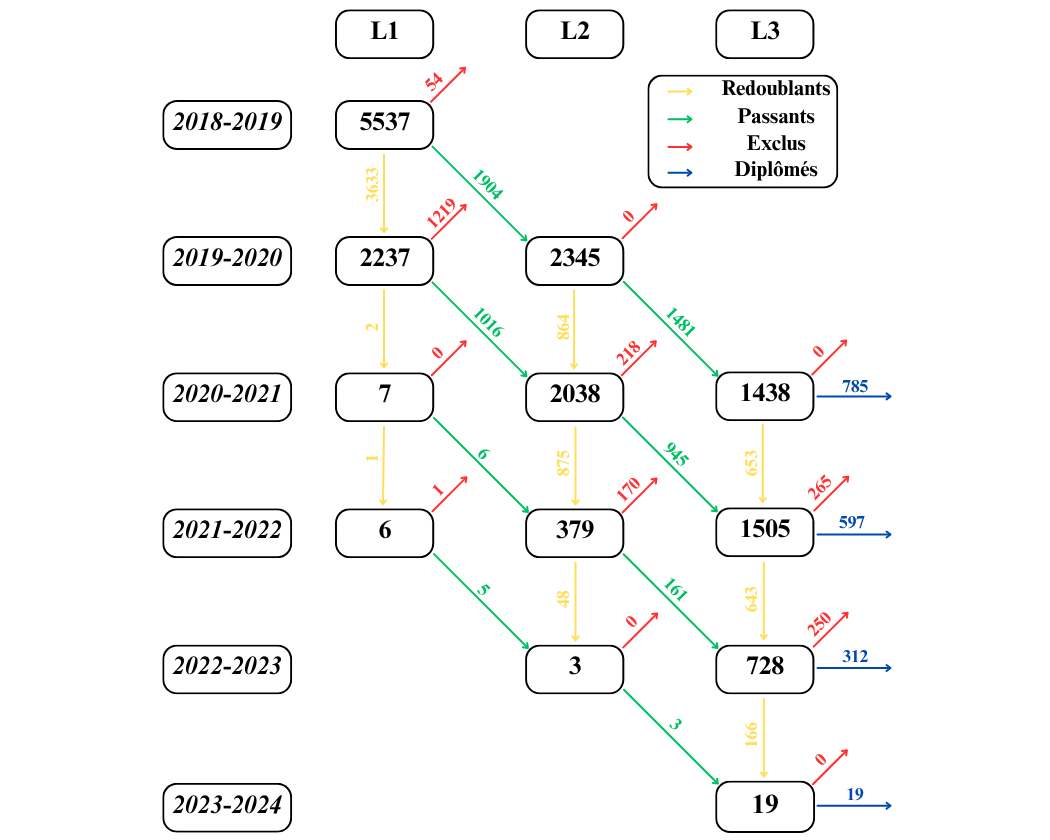
\includegraphics[width=1\textwidth]{figure/L1_2018.png}
\end{figure}

\newpage
\subsubsection{cohorte 2018(S2)}

\begin{figure}[ht]
    \centering
    \caption{Graphe suivi de la cohorte 2018 (S2)}
    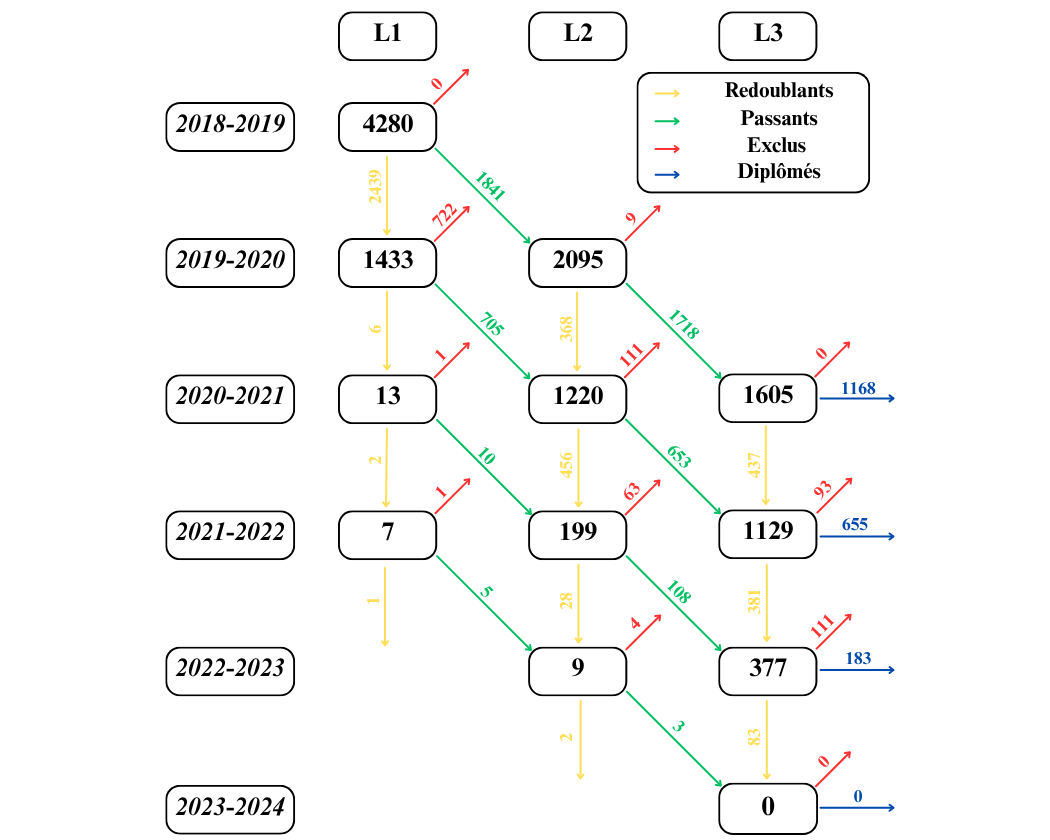
\includegraphics[width=1\textwidth]{figure/S2_2018.png}
\end{figure}

\newpage
\subsubsection{cohorte 2018(S1)}

\begin{figure}[ht]
    \centering
    \caption{Graphe suivi de la cohorte 2018 (S1)}
    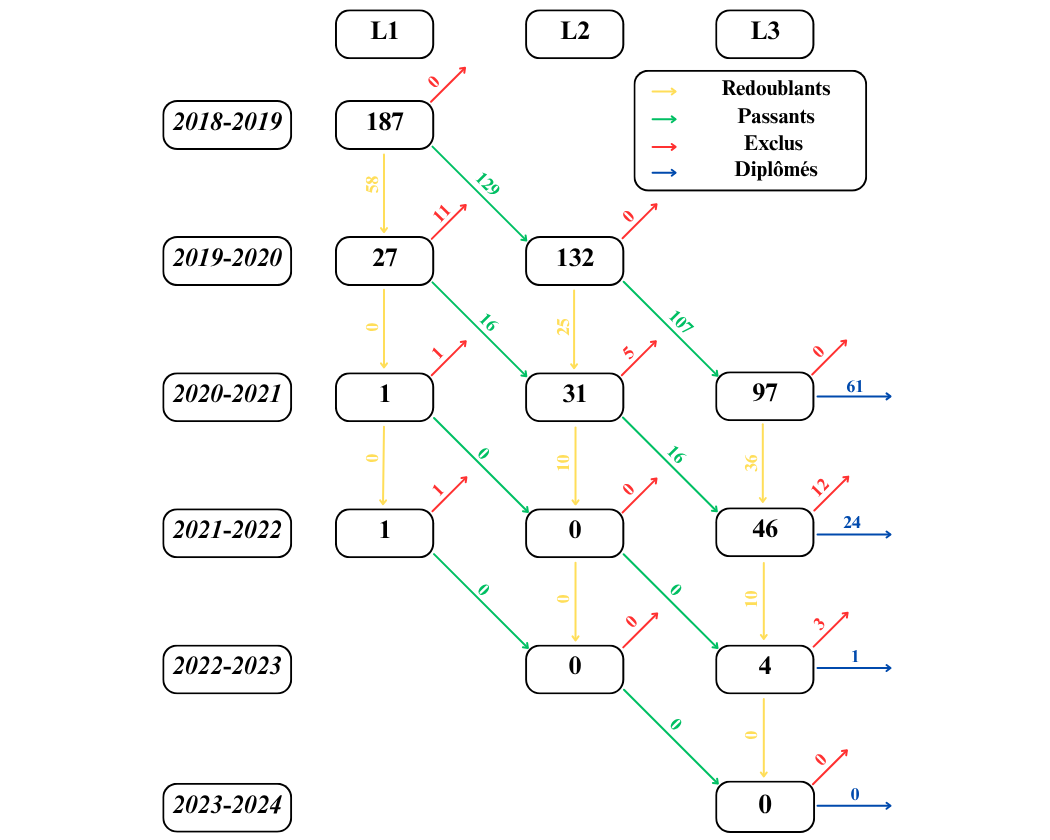
\includegraphics[width=1\textwidth]{figure/S1_2018.png}
\end{figure}

\newpage
\subsection{Série STEG et G}

\subsubsection{cohorte 2019(STEG)}

\begin{figure}[ht]
    \centering
    \caption{Graphe suivi de la cohorte 2019 (STEG)}
    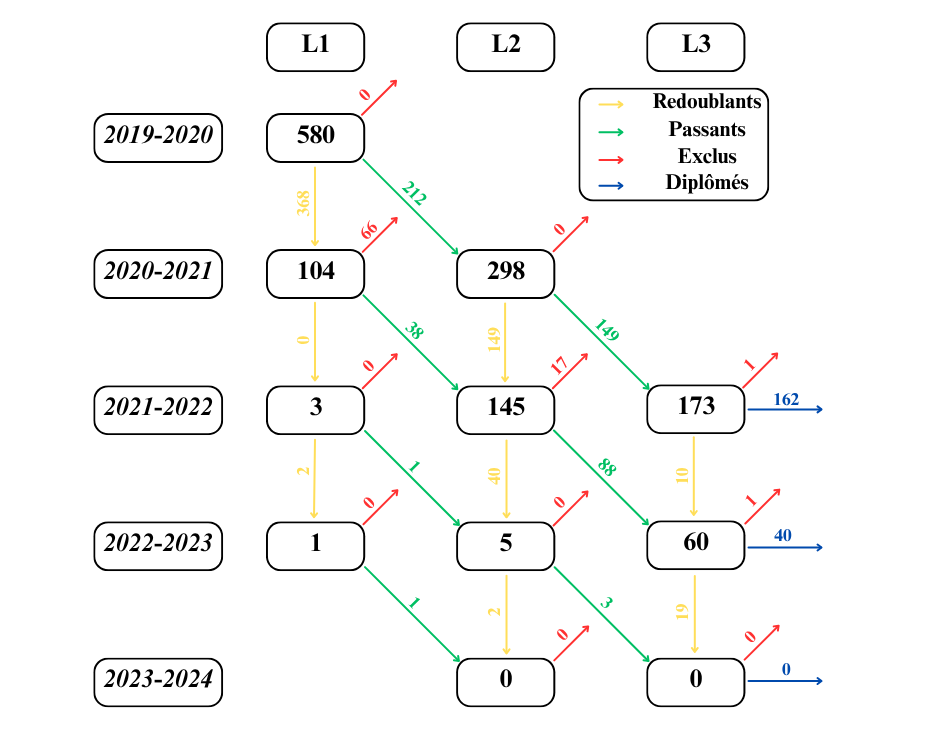
\includegraphics[width=1\textwidth]{figure/STEG_2019.png}
\end{figure}

\newpage
\subsubsection{cohorte 2018(G)}

\begin{figure}[ht]
    \centering
    \caption{Graphe suivi de la cohorte 2018 (G)}
    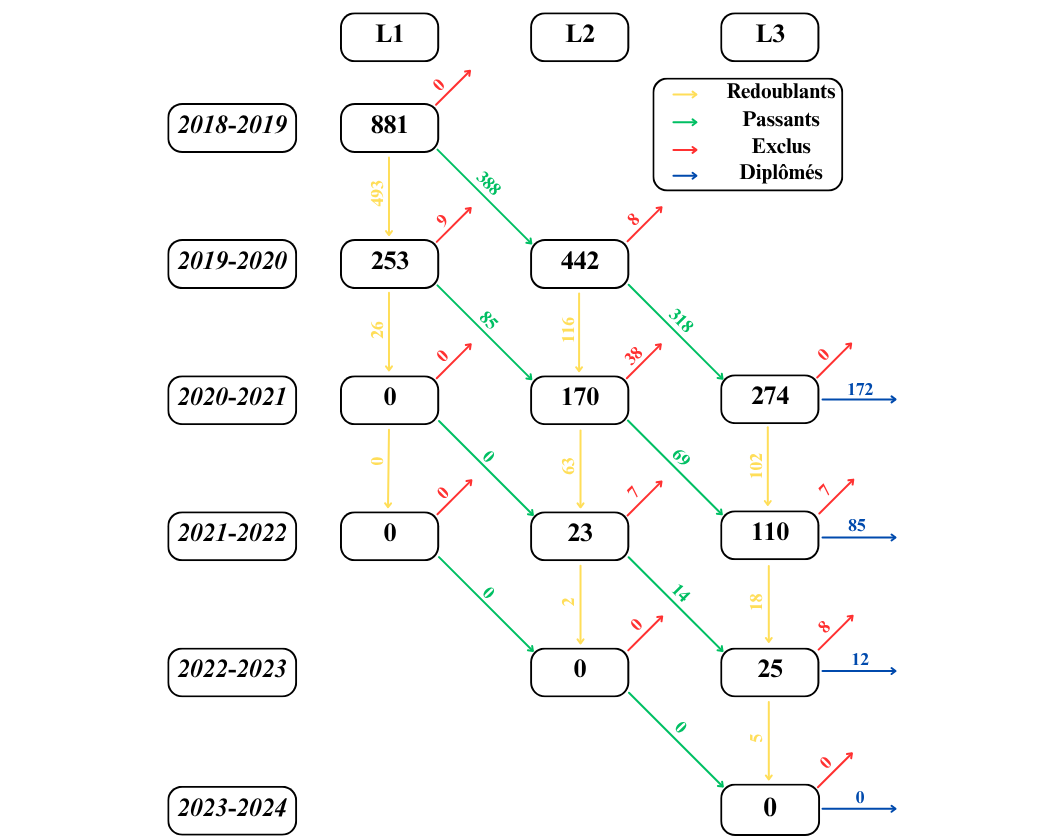
\includegraphics[width=1\textwidth]{figure/G_2018.png}
\end{figure}

\newpage

\section{Analyse des performances académiques}
\section{Conclusion}